\begin{figure}[H]
  \centering
  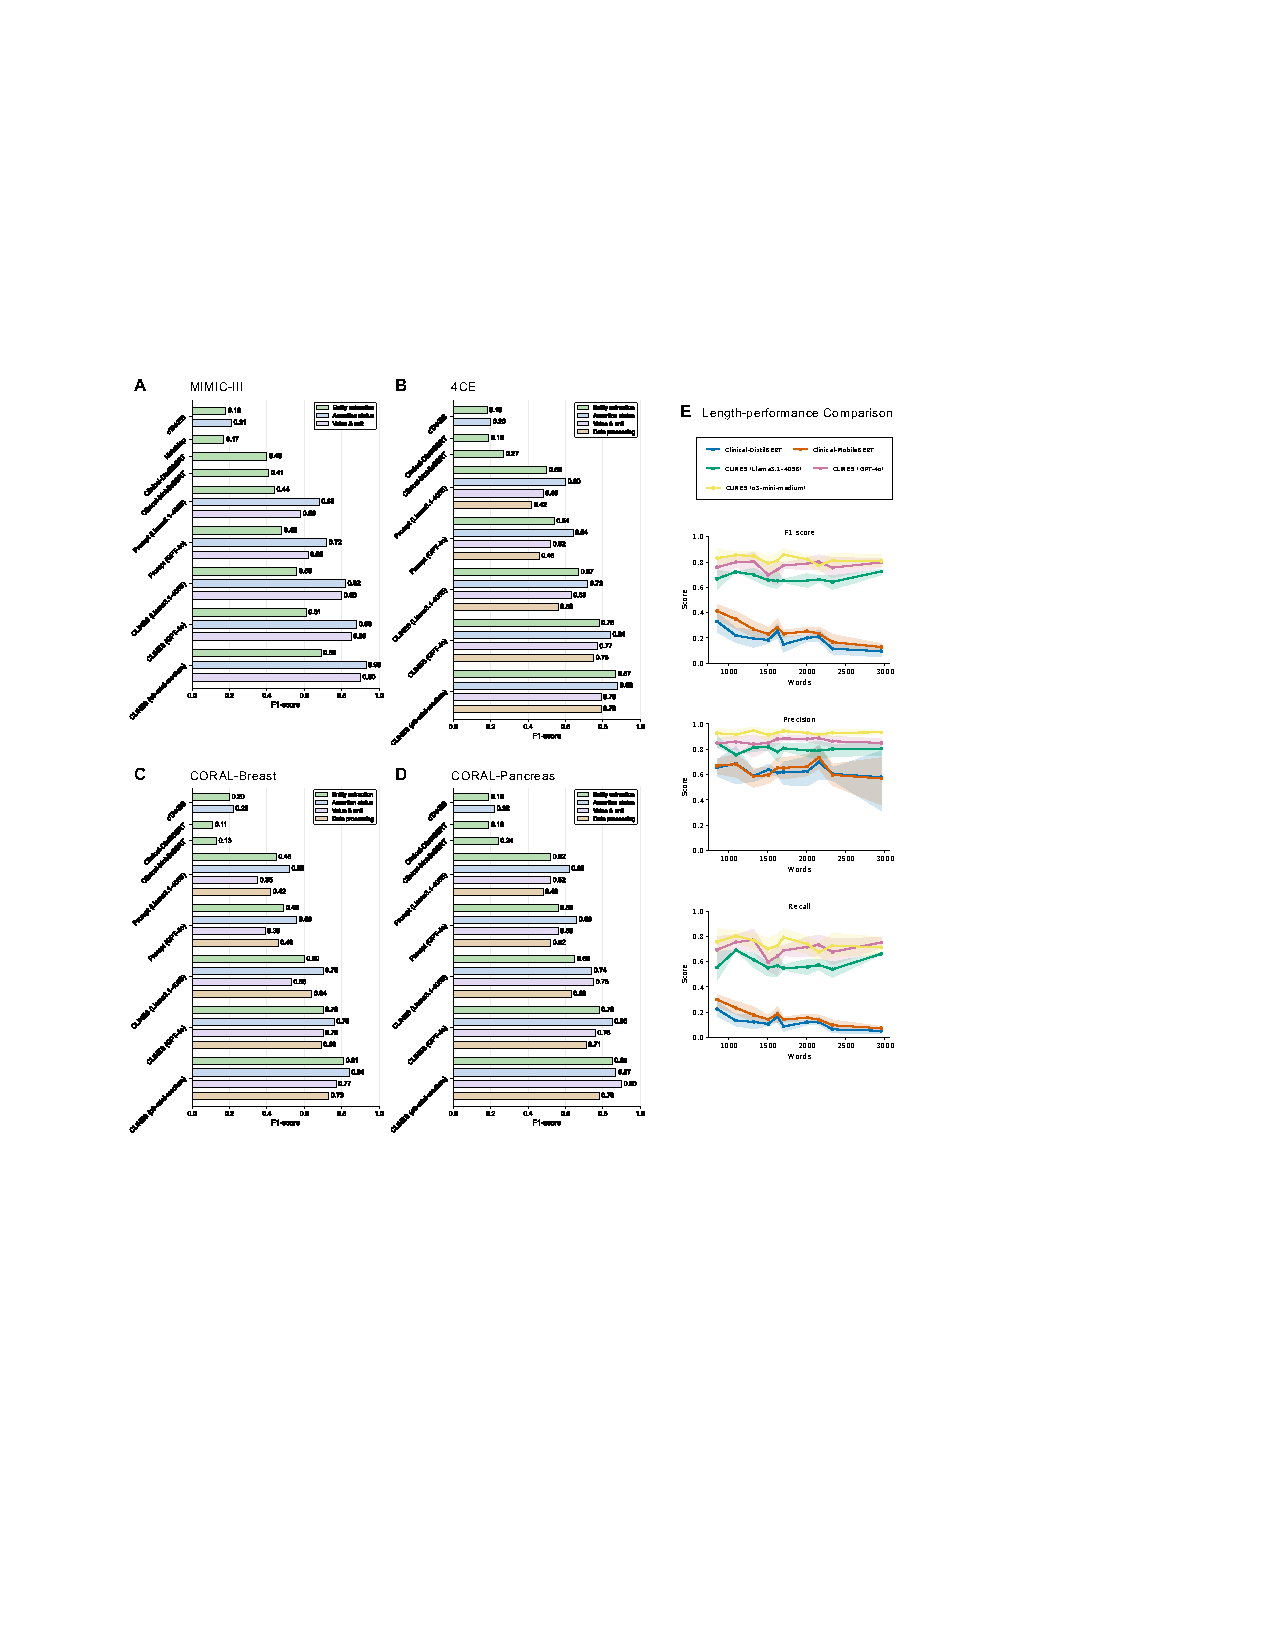
\includegraphics[width=\linewidth]{figures/figure3.pdf}
  \caption{\textbf{Performance of CLINES across datasets and tasks.} (A--D) Results on MIMIC-III, 4CE, and CORAL---Breast/Pancreas comparing CLINES with traditional rule-based NLP, lightweight transformer-based baselines, and LLMs with single-step prompt engineering across six extraction tasks (treating value+unit as a single field and evaluating start+end date as joint correctness). The metric is F1 score. (E) CLINES versus transformer-based baselines as note length/complexity increases, reported as F1, precision, and recall. Notes are grouped into quantile-based length bins; markers indicate the bin-median word count; lines show bin-mean scores; shaded ribbons denote 95\% bootstrap confidence intervals.}
  \label{fig:clines-performance}
\end{figure}
